\documentclass[11pt]{article}
\usepackage[T1]{fontenc}
\usepackage[utf8]{inputenc}
\usepackage{lmodern}
\usepackage[margin=1in]{geometry}
\usepackage{amsmath,amssymb,amsthm,mathtools,bm}
\usepackage{booktabs,enumitem,graphicx,xcolor,microtype}
\usepackage{tikz,xurl}
\usetikzlibrary{arrows.meta,positioning,calc}
\usepackage[colorlinks=true,linkcolor=blue!55!black,citecolor=blue!55!black,urlcolor=blue!55!black]{hyperref}
\usepackage[capitalise,noabbrev]{cleveref}
\numberwithin{equation}{section}
\newtheorem{theorem}{Theorem}[section]
\newtheorem{lemma}[theorem]{Lemma}
\newtheorem{proposition}[theorem]{Proposition}
\newtheorem{corollary}[theorem]{Corollary}
\theoremstyle{definition}
\newtheorem{definition}[theorem]{Definition}
\theoremstyle{remark}
\newtheorem{remark}[theorem]{Remark}
\newcommand{\R}{\mathbb R}
\newcommand{\C}{\mathbb C}
\newcommand{\D}{\mathbb D}
\newcommand{\ddc}{dd^c}
\newcommand{\dc}{d^c}
\newcommand{\vol}{\operatorname{vol}}
\newcommand{\interior}{\operatorname{int}}
\newcommand{\ip}[2]{\langle #1,#2\rangle}
\newcommand{\norm}[1]{\lVert #1\rVert}
\title{Symplectic Balls in Symmetric Polar Products}
\author{OpenAI}
\date{September 22, 2026}
\hypersetup{pdftitle={Symplectic Balls in Symmetric Polar Products},pdfauthor={OpenAI},pdfsubject={Gromov width and the symmetric Mahler conjecture}}
\begin{document}
\maketitle
\begin{abstract}
For every integer $n\ge2$ and every origin-symmetric convex body
$K\subset\R^n$, we prove that the Gromov width of
$\interior K\times\interior K^\circ$ is $4$.
We construct smooth symplectic embeddings of standard balls of every
capacity $0<c<4$ into this polar product.
Volume preservation then resolves the symmetric Mahler conjecture positively
in every dimension.
\end{abstract}
\section{Introduction}\label{sec:introduction}

Let $K\subset\R^n$ be an origin-symmetric convex body: a compact convex
set with nonempty interior and $K=-K$. Its polar is
\[
 K^\circ=\{p\in\R^n:\ip{q}{p}\le1\text{ for every }q\in K\}.
\]
We place $K$ in the position coordinates and $K^\circ$ in the conjugate
momentum coordinates of $(\R^n_q\times\R^n_p,\omega_0)$, where
\[
 \omega_0=\sum_{j=1}^n dq_j\wedge dp_j,
 \qquad U_K=\interior K\times\interior K^\circ.
\]
For $c>0$, write
\[
 B^{2n}(c)=\{(q,p):\pi(|q|^2+|p|^2)<c\}.
\]
The Gromov width $c_G(U)$ of an open set $U\subset\R^{2n}$ is the supremum
of the capacities $c$ for which there is a smooth embedding
$e:B^{2n}(c)\to U$ satisfying $e^*\omega_0=\omega_0$.

\begin{theorem}\label{thm:main}
For every integer $n\ge2$ and every origin-symmetric convex body
$K\subset\R^n$,
\[
 c_G(U_K)=4.
\]
More precisely, for every $0<c<4$ there is a smooth symplectic embedding
$B^{2n}(c)\hookrightarrow U_K$.
\end{theorem}

The theorem imposes no smoothness, strict convexity, unconditional
symmetry, or product structure on $K$. It concerns every capacity
strictly below $4$; no embedding at the supremum is needed.
Symplectic embeddings preserve volume, and
$\vol_{2n}(B^{2n}(c))=c^n/n!$. Consequently Theorem~\ref{thm:main}
gives
\[
 \vol_n(K)\vol_n(K^\circ)\ge\frac{4^n}{n!}.
\]
Thus the theorem resolves the symmetric Mahler conjecture positively;
the complete deduction, including the one-dimensional case, appears in
Corollary~\ref{cor:mahler}. We make no claim here about the classification
of equality cases.

For $n\ge3$, the width theorem also transports finite ball packings
satisfying strict volume and pairwise-capacity inequalities into $U_K$; see
Corollary~\ref{cor:polar-packings}.

\subsection*{Background and prior constructions}

The symmetric volume-product problem goes back to Mahler's work on
transference in the geometry of numbers \cite{Mahler1939}.
Earlier sharp volume inequalities cover the plane
\cite[Theorem~13]{BoroczkyMakaiMeyerReisner2013}, unconditional bodies
(those invariant under coordinate sign changes)
\cite[Sections~1--2]{Reisner1987}, and dimension three
\cite{IriyehShibata}. Bourgain and Milman's asymptotic reverse
Santal\'o inequality gives a lower bound $a^n/n!$ for some $a>0$
independent of dimension \cite{BourgainMilman}; the sharp target is
$4^n/n!$. The companion paper \cite{SymmetricCompanion2026} discusses
the wider convex-geometric history and the equality problem. Our focus
is the stronger geometric assertion that the polar product contains
large symplectic balls.

Gromov's nonsqueezing theorem established that ball embeddings detect
symplectic restrictions beyond volume preservation \cite{Gromov1985}.
Viterbo later proposed a sharp volume--capacity inequality for convex
domains \cite{Viterbo2000}. Artstein-Avidan, Karasev, and Ostrover
connected this proposed inequality to the symmetric Mahler conjecture
and proved
\[
 c_{\mathrm{HZ}}(K\times K^\circ)=4
\]
for every origin-symmetric convex body
\cite[Theorems~1.6--1.7 and Section~4]{AAKO2014}.
Here $c_{\mathrm{HZ}}$ is the Hofer--Zehnder capacity, normalized to
have value $\pi R^2$ on a ball of radius $R$
\cite{HoferZehnder1994}. This computation implies the upper bound for
Gromov width. We use the supporting-cylinder argument of
\cite[Remark~4.2]{AAKO2014} and nonsqueezing to prove that bound directly.
The matching lower bound requires actual ball embeddings; it does not
follow from the Hofer--Zehnder capacity computation.

Earlier constructions establish this lower bound for particular
families. Karasev proves it for $\ell_p$ unit balls, $1<p<\infty$,
\cite[Proposition~3.1]{Karasev2021}, using coordinatewise area-preserving
constructions related to those of Latschev, McDuff, and Schlenk
\cite{LatschevMcDuffSchlenk2013}. Ramos and Sepe identify the interior of
the cube--crosspolytope product with the open ball of capacity $4$
\cite[Theorem~7]{RamosSepe2019}. Vicente obtains capacity equalities
for functional-dual products defined by Young functions and lower
bounds for ordinary polar products
\cite[Theorems~1.3 and~1.5]{Vicente2025}.
Functional duality and ordinary polarity give different partners, so
these results require separate hypotheses. Theorem~\ref{thm:main}
answers positively the unrestricted symmetric-polar-product width
question formulated in \cite{VicenteQuestion2026}.

The unrestricted Viterbo volume--capacity conjecture was disproved by
Haim-Kislev and Ostrover \cite{HKO2025}. Their four-dimensional
counterexample uses a regular pentagon and a rotated partner
\cite[Theorem~1.3 and Proposition~1.4]{HKO2025}; the pentagon is not
centrally symmetric. The theorem here concerns the particular
Lagrangian product of a symmetric body and its polar, and makes no
assertion for arbitrary convex domains in phase space.

The planar coordinate is Gross's uniform-distribution map in the
conformal Skorokhod construction, rotated in source and target
\cite[Section~3.2]{Gross2019}. The same lens and high powers of its
inverse coordinate appear in the complete companion paper
\cite[Section~3 and proof of Lemma~5.1]{SymmetricCompanion2026}.
Every lens estimate needed here, including the estimate uniform up to
the tips, is proved locally.
Neither the volume-product theorem nor the equality classification of
the companion is used in the proof.

The holomorphic-zero argument belongs to the broader use of logarithmic
poles to measure local positivity, as in Demailly
\cite[Section~6]{Demailly1992}. Its replacement of a potential near the
origin by a regularized maximum has a close analogue in Witt Nystr\"om
\cite[Proposition~3.3]{WittNystrom2018}. Those results concern projective
K\"ahler geometry; here the replacement is proved directly for the
specified form on a noncompact sublevel domain. Moser's deformation
method \cite[Section~4]{Moser1965}, with compact support verified below,
then transfers the ball to the original form. The radial coordinate
change is a special case of the K\"ahler symplectic-coordinate formula of
Loi and Zuddas \cite[proof of Theorem~1.1, equation~(23)]{LoiZuddas2008};
its pullback is also verified directly.


\subsection*{The construction}

The lower bound comes from comparing two scales. For a fixed body $K$
given by finitely many symmetric strips and a large integer $k$, a
holomorphic construction produces balls of every capacity below $\pi k$ in a suitable symplectic
domain. We realize that domain in
$\interior K\times S_k\interior K^\circ$, where the momentum scale
satisfies $S_k=(1+o(1))\pi k/4$ as $k\to\infty$.
Dividing momentum by $S_k$ and compensating with a dilation of the
source ball gives each prescribed capacity below $4$ once $k$ is
sufficiently large.
Two independent analytic ingredients supply these scales.

The first turns holomorphic vanishing into a ball
(Theorem~\ref{thm:holomorphic-ball}). Let $f=(f_1,\ldots,f_m)$ be holomorphic on an open set
$\Omega\subset\C^n$ containing $0$, have the unique common zero $0$,
and satisfy
$|f(z)|=O(|z|^k)$ there. The domain $\{|f|^2<1\}$, equipped with a symplectic form
constructed from the potential $|z|^2+|f(z)|^2$, contains balls of every
capacity strictly below $\pi k$, provided the closed sublevels of
$|f|^2$ below $1$ are compact in $\Omega$. The order of vanishing controls the
slope of a logarithmic potential near zero. Replacing its singularity
by a smooth radial potential exposes a ball, and a compactly supported
Moser deformation transports that ball to the original form.
Compact sublevels ensure the deformation is supported away from the
boundary; no regularity of the level hypersurfaces is required.

The second ingredient controls the momentum scale
(Proposition~\ref{prop:uniform-slice}). A conformal map $F$ takes the unit
disk $\D=\{w\in\C:|w|<1\}$ to a bounded domain $D$ with tips at $\pm i$
and centered horizontal slices at every height $-1<t<1$.
Write $g=F^{-1}$. The horizontal primitives of the densities
$|(g^k)'|^2$, taken from the imaginary axis, have absolute value at most
$(\pi k/4)|g|^{2k}+o(k)$, uniformly on all of $D$. Uniformity near the tips is essential:
the slice height may approach $1$ or $-1$ as $k$ increases.
Section~\ref{sec:planar} proves this estimate locally, including the
moving-endpoint bound needed at those tips.

To combine the ingredients, write
$K=\{x:|\langle b_j,x\rangle|\le1,\ 1\le j\le m\}$, where the real
vectors $b_j$ span $\R^n$. Extend these pairings complex-linearly and
set $f_j(z)=g(\langle b_j,z\rangle)^k$ on the domain where every
$\langle b_j,z\rangle$ lies in $D$. These functions have the required
unique common zero and compact sublevels. The phase-space realization
sends the imaginary part of $z$ to position and uses the horizontal
primitives for momentum. Their monotonicity makes the map globally
injective, and their uniform estimate bounds the momentum in the polar
body. Section~\ref{sec:realization} carries out this construction.
Finally, approximation in the polar body extends the lower bound to
arbitrary $K$. A supporting-cylinder argument and nonsqueezing give
the matching upper bound.

\subsection*{Organization}

Section~\ref{sec:ball} proves the holomorphic ball principle.
Section~\ref{sec:planar} constructs the planar coordinate and proves the
uniform slice estimate. Section~\ref{sec:realization} treats finite strip
bodies, and Section~\ref{sec:approximation} passes to all convex bodies,
proves the matching upper bound, and derives the volume-product and
packing consequences.
Balls and symplectic domains are open unless explicitly stated otherwise.

\section{Balls from holomorphic vanishing}
\label{sec:ball}

The aim of this section is to turn the order of a holomorphic zero into
the capacity of an embedded ball. We first fix the differential-form
normalization, then smooth a logarithmic singularity and transport the
resulting radial ball by Moser's deformation method.

Identify $\C^n$ with $\R^{2n}$ by writing $z=u+ix$.  For a smooth real
function $\phi$, use the convention
\[
 \dc\phi(X)=-\frac14\,d\phi(iX),
 \qquad \ddc\phi=d(\dc\phi).
\]
In particular, the standard primitive and symplectic form are
\begin{equation}
 \lambda_0=\dc|z|^2
   =\frac12\sum_{j=1}^n(u_j\,dx_j-x_j\,du_j),
 \qquad
 \omega_0=\ddc|z|^2=\sum_{j=1}^n du_j\wedge dx_j.
 \label{eq:ball-normalization}
\end{equation}
For every real tangent vector $X$, one has
\[
 \ddc\phi(X,iX)
 =\frac14\left.\Delta_{\zeta}\phi(z+\zeta X)\right|_{\zeta=0},
 \qquad \zeta\in\C.
\]
Thus a smooth function $\phi$ is plurisubharmonic precisely when these
quantities are nonnegative.  In that case $\ddc(|z|^2+\phi)$ is symplectic:
it is closed and its value on $(X,iX)$ is at least $|X|^2$.

We will also use that a smooth convex, coordinatewise nondecreasing
function of plurisubharmonic functions is plurisubharmonic.  Indeed, on
each complex line the ordinary chain rule gives
\[
 \Delta\Gamma(h_1,\ldots,h_N)
 =\sum_{j=1}^N\Gamma_j\Delta h_j
   +\sum_{i,j=1}^N\Gamma_{ij}
        \ip{\nabla h_i}{\nabla h_j}\ge0.
\]
The first sum is nonnegative by monotonicity, and the second is
nonnegative because the Hessian of $\Gamma$ is positive semidefinite.

\begin{theorem}[A ball from a holomorphic zero]
\label{thm:holomorphic-ball}
Let $n,m\ge1$, let $\Omega\subset\C^n$ be an open set containing $0$,
and let $f=(f_1,\ldots,f_m):\Omega\to\C^m$ be holomorphic.  Suppose that,
for some integer $k\ge1$,
\begin{enumerate}[label=\textup{(\roman*)}]
 \item $f^{-1}(0)=\{0\}$ and $|f(z)|=O(|z|^k)$ as $z\to0$;
 \item for every $0<s<1$, the set
 $\{z\in\Omega:|f(z)|^2\le s\}$ is a compact subset of $\Omega$.
\end{enumerate}
Set
\[
 \tau=|f|^2,\qquad V=\{z\in\Omega:\tau(z)<1\},
 \qquad \omega=\ddc(|z|^2+\tau).
\]
For every $0<c<\pi k$, there is a smooth symplectic embedding
\[
 \bigl(B^{2n}(c),\omega_0\bigr)\longrightarrow(V,\omega).
\]
\end{theorem}

\begin{proof}
\noindent\textit{Step 1: a logarithmic potential with the required slope.}
For a holomorphic tuple, differentiation along a complex line gives
\begin{align}
 \ddc\tau(X,iX)&=|df(X)|^2,\notag\\
 \ddc\log\tau(X,iX)
 &=\frac{|f|^2|df(X)|^2
       -\left|\sum_{j=1}^m\overline{f_j}\,df_j(X)\right|^2}{|f|^4}
 \quad\text{on }\Omega\setminus\{0\}.
 \label{eq:ball-log-levi}
\end{align}
The second expression is nonnegative by Cauchy--Schwarz.  Hence $\tau$
and, away from its zero, $\log\tau$ are plurisubharmonic.

Fix $0<a<k$; we will embed the ball of capacity $\pi a$.  Choose
\[
 \frac ak<b<1,\qquad a<\mu<bk.
\]
Choose numbers $\log b<t_-<t_+<0$ and a smooth nondecreasing cutoff
$\beta:\R\to[0,1]$ which is $0$ for $t\le t_-$ and $1$ for $t\ge t_+$.
Define $\chi$ on $(-\infty,0)$ by
\[
 \chi'(t)=b+\beta(t)(e^t-b),
\]
choosing its additive constant so that $\chi(t)=e^t$ for $t\ge t_+$.
This is possible since $\chi'=e^t$ there.  Moreover, $\chi'>0$ and
\[
 \chi''(t)=\beta'(t)(e^t-b)+\beta(t)e^t\ge0,
\]
because the transition occurs where $e^t>b$.  For $t\le t_-$, the
function $\chi$ is affine with slope $b$.

It follows that
\[
 H=\chi(\log\tau)
\]
is smooth and plurisubharmonic on $V\setminus\{0\}$ and satisfies
$H=\tau$ wherever $\tau\ge s_0:=e^{t_+}$.  The vanishing assumption gives
$\tau(z)\le C_0|z|^{2k}$ near zero.  Since $\chi$ is eventually affine,
there is a constant $C_1$ such that
\begin{equation}
 H(z)\le bk\log|z|^2+C_1
 \quad\text{for all sufficiently small }z\ne0.
 \label{eq:ball-singularity}
\end{equation}

\medskip
\noindent\textit{Step 2: smooth the singularity without changing the form near the boundary.}
The strict inequality $\mu<bk$ lets a smooth radial logarithm dominate
$H$ close to zero while remaining below it on an outer sphere.
Write $B_r=\{z\in\C^n:|z|<r\}$, and choose $r_2>0$ with
$\overline{B}_{r_2}\subset V$.  For $0<\delta\le1$, consider
\[
 P_\delta(z)=\mu\log(|z|^2+\delta)-M.
\]
For each fixed $r>0$, the radial calculation in Step~4 identifies
$(B_r,\ddc(|z|^2+P_\delta))$ with a standard ball whose squared radius
is $r^2+\mu r^2/(r^2+\delta)$. Since $\mu>a$, this exceeds $a$ for
all sufficiently small $\delta$. We will therefore arrange that the
modified potential agrees with $P_\delta$ on a ball whose radius is
fixed before $\delta$ is chosen.

The functions $P_\delta$ are plurisubharmonic by
Equation~\eqref{eq:ball-log-levi}, applied to the nowhere-zero
holomorphic tuple $(\sqrt\delta,z_1,\ldots,z_n)$.  Choose $M$ so that
\[
 M>\mu\log(r_2^2+1)-\min_{|z|=r_2}H(z)+2.
\]
The minimum is finite because $f$ has no zero on this sphere.  Then
$P_\delta<H-2$ on $|z|=r_2$ for every $0<\delta\le1$.
On the other hand, Equation~\eqref{eq:ball-singularity} gives
\[
 P_\delta(z)-H(z)
 \ge(\mu-bk)\log|z|^2-M-C_1.
\]
As $z\to0$, this lower bound tends to $+\infty$, uniformly in $\delta$.
We may therefore fix $0<r_1<r_2$, independently of $\delta$, such that
\begin{equation}
 P_\delta>H+2\quad\text{on }0<|z|\le r_1
 \quad\text{for every }0<\delta\le1.
 \label{eq:ball-inner-domination}
\end{equation}
Fix from now on one positive $\delta$ satisfying
\begin{equation}
 0<\delta<\min\left\{1,\ r_1^2\left(\frac\mu a-1\right)\right\}.
 \label{eq:ball-delta-choice}
\end{equation}
The upper bound is positive because $\mu>a$.

We next replace the singularity of $H$ by $P_\delta$ using a
regularized maximum, the standard gluing device in Richberg's smoothing
method; see \cite[Section~2]{HarveyLawsonPlis2020}. A related replacement
of K\"ahler potentials appears in
\cite[Proposition~3.3]{WittNystrom2018} in a projective setting.
We give the elementary two-function construction explicitly. Let
$\vartheta\in C_c^\infty((-1,1))$ be nonnegative and even, with
$\int_{\R}\vartheta=1$, and set
\[
 \rho(s)=\int_{\R}|s-t|\vartheta(t)\,dt,
 \qquad
 \operatorname{rmax}(h,p)=\frac{h+p+\rho(h-p)}2.
\]
The function $\rho$ is smooth and convex, with $|\rho'|\le1$, and
equals $|s|$ for $|s|\ge1$.  Thus $\operatorname{rmax}$ is smooth,
convex, nondecreasing in both arguments, and equals $\max(h,p)$ when
$|h-p|\ge1$.  Define $\widetilde H$ to be
$\operatorname{rmax}(H,P_\delta)$ on $B_{r_2}\setminus\{0\}$, to be
$H$ outside $B_{r_2}$, and to take the value $P_\delta(0)$ at zero.
The outer comparison gives equality with $H$ in a neighborhood of
$\partial B_{r_2}$, and Equation~\eqref{eq:ball-inner-domination} gives
equality with $P_\delta$ on $B_{r_1}$.  Consequently $\widetilde H$ is
smooth and plurisubharmonic on all of $V$.

The difference $\widetilde H-\tau$ has compact support in $V$.
Indeed, set $s_2=\max_{\overline B_{r_2}}\tau<1$, choose
$\max(s_0,s_2)<\sigma<1$, and put
\begin{equation}
 C=\{z\in\Omega:\tau(z)\le\sigma\}.
 \label{eq:ball-support}
\end{equation}
This is a compact subset of $V$ by hypothesis.  Outside $C$ a point
lies outside $\overline B_{r_2}$ and has $H=\tau$, so that
$\widetilde H-\tau$ vanishes there.

\medskip
\noindent\textit{Step 3: transport the smoothed form.}
We now use Moser's deformation argument \cite[Section~4]{Moser1965}.
The support estimate above supplies a complete flow even though $V$
need not be compact. Consider the symplectic forms
\[
 \omega_s=\ddc\bigl(|z|^2+(1-s)\tau+s\widetilde H\bigr),
 \qquad 0\le s\le1,
\]
and write $\widetilde\omega=\omega_1$.  Each form is symplectic because
the two non-Euclidean potentials are plurisubharmonic.  Define the
smooth time-dependent vector field $Y_s$ by
\[
 \iota_{Y_s}\omega_s=-\gamma,
 \qquad \gamma=\dc(\widetilde H-\tau).
\]
Both $\gamma$ and every $Y_s$ are supported in the fixed compact set
$C$.  Extending $Y_s$ by zero outside $V$ gives a smooth vector field
on $\C^n$, with its coefficients and first derivatives bounded
uniformly for $s\in[0,1]$.  The ordinary differential equation for
this field has a flow $\varphi_s$ throughout this time interval.
The ambient flow fixes $\C^n\setminus V$ pointwise and hence restricts
to diffeomorphisms of $V$.  This argument applies even if $V$ is
disconnected and places no regularity assumption on its boundary.

Since $d\omega_s=0$, differentiation of pullbacks gives
\[
 \frac{d}{ds}\varphi_s^*\omega_s
 =\varphi_s^*\bigl(d\gamma+d\iota_{Y_s}\omega_s\bigr)=0.
\]
Therefore
\begin{equation}
 \varphi_1^*\widetilde\omega=\omega,
 \qquad
 \varphi_1^{-1}:(V,\widetilde\omega)\longrightarrow(V,\omega)
 \text{ is symplectic}.
 \label{eq:ball-moser}
\end{equation}

\medskip
\noindent\textit{Step 4: read off the ball in the radial model.}
The deformation has reduced the problem to an explicit radial form.
On $B_{r_1}$ the new potential, up to the additive constant $-M$, is
$\Psi(|z|^2)$, where
\[
 \Psi(t)=t+\mu\log(t+\delta).
\]
Define the radial map
\[
 R(z)=\sqrt{\Psi'(|z|^2)}\,z
     =\sqrt{1+\frac\mu{|z|^2+\delta}}\,z.
\]
This is the radial case of the symplectic-coordinate construction in
\cite[proof of Theorem~1.1, Equation~(23)]{LoiZuddas2008}.
In the pullback of $\lambda_0$ from
Equation~\eqref{eq:ball-normalization}, the terms differentiating the
radial factor cancel.  Hence
\[
 R^*\lambda_0=\Psi'(|z|^2)\lambda_0=\dc\Psi(|z|^2),
 \qquad R^*\omega_0=\widetilde\omega\big|_{B_{r_1}}.
\]
The squared radial coordinate is strictly increasing, because
\[
 \frac{d}{dt}\bigl(t\Psi'(t)\bigr)
 =\frac{d}{dt}\left(t+\frac{\mu t}{t+\delta}\right)
 =1+\frac{\mu\delta}{(t+\delta)^2}>0.
\]
At zero the map is smooth and has derivative
$DR(0)=\sqrt{1+\mu/\delta}\,I$, so its inverse is smooth there as
well.  Thus $R$ is a diffeomorphism from $B_{r_1}$ onto the standard
ball $B^{2n}(\pi Q_\delta)$, where
\[
 Q_\delta=r_1^2+\frac{\mu r_1^2}{r_1^2+\delta}>a
\]
by Equation~\eqref{eq:ball-delta-choice}.  If
$\iota:B_{r_1}\hookrightarrow V$ denotes inclusion, the map
\[
 \varphi_1^{-1}\circ\iota\circ
       R^{-1}\big|_{B^{2n}(\pi a)}:
 B^{2n}(\pi a)\longrightarrow V
\]
is a smooth embedding, and its pullback of $\omega$ is $\omega_0$ by
Equation~\eqref{eq:ball-moser} and the radial pullback identity.
Since $a$ was arbitrary in $(0,k)$, the theorem follows.
\end{proof}

\section{A planar coordinate and a uniform slice estimate}
\label{sec:planar}

We use Gross's conformal map $\psi$ for the uniform distribution
\cite[Section~3.2]{Gross2019}, with the rotation $F(w)=i\psi(iw)$.
There is no scaling. The same lens appears in
\cite[Section~3]{SymmetricCompanion2026}; its half-width $\lambda(t)$
is the function $V(t)$ used here. We establish its needed properties
directly and then prove a uniform slice estimate that controls the
momentum coordinates in the polar product.

\begin{lemma}\label{lem:planar-map}
The holomorphic function
\begin{equation}\label{eq:planar-F}
 F(w)=\frac{8}{\pi^2}\sum_{\ell=0}^{\infty}
       \frac{(-1)^\ell w^{2\ell+1}}{(2\ell+1)^2},
 \qquad w\in\D,
\end{equation}
is a biholomorphism from \(\D\) onto a bounded domain \(D\).
It is odd, commutes with conjugation, and satisfies \(F(0)=0\).
The imaginary coordinates of \(D\) range over \((-1,1)\), and for each
\(t\in(-1,1)\) there is a finite \(V(t)>0\) such that
\begin{equation}\label{eq:horizontal-slices}
 \{v\in\R:v+it\in D\}=(-V(t),V(t)).
\end{equation}
Write \(F(ir)=iT(r)\) for \(0\le r<1\).  The function \(T\) increases
strictly from \(0\) to \(1\), with
\begin{equation}\label{eq:planar-T}
 T'(r)=\frac{8}{\pi^2}\frac{\operatorname{arctanh}r}{r}
 \quad(0<r<1),
 \qquad \lim_{r\uparrow1}T'(r)=+\infty.
\end{equation}
For fixed \(t\in(-1,1)\), put \(r_0=T^{-1}(|t|)\).  The positive
horizontal slice is parametrized by
\[
 w(r,t)=re^{i\theta(r,t)},\qquad
 F(w(r,t))=v(r,t)+it,\qquad r_0<r<1,
\]
where \(-\pi/2<\theta(r,t)<\pi/2\) and \(v(r,t)\) increases strictly
from \(0\) to \(V(t)\).
\end{lemma}

\begin{proof}
\noindent\textit{The map and its angular derivative.}
The series in Equation~\eqref{eq:planar-F} is absolutely summable on the
closed disk.  Hence \(F\) is bounded, odd, and commutes with conjugation.
Termwise differentiation in the open disk gives
\begin{equation}\label{eq:planar-arctan}
 wF'(w)=\frac{8}{\pi^2}\arctan w,
 \qquad
 \arctan w=\frac{1}{2i}\log\frac{1+iw}{1-iw}.
\end{equation}
Here the logarithm is the branch on the right half-plane that is real on
the positive real axis.  Indeed,
\[
 \Re\frac{1+iw}{1-iw}
   =\frac{1-|w|^2}{|1-iw|^2}>0
 \qquad (w\in\D).
\]
This also shows that \(\arctan w=0\) only at \(w=0\).
Thus \(F'\) has no zeros away from the origin, and the series gives
\(F'(0)=8/\pi^2\ne0\).

For \(w=re^{i\theta}\), define
\begin{equation}\label{eq:planar-A}
 A(r,\theta)=\Re\bigl(wF'(w)\bigr)
   =\frac{4}{\pi^2}
       \arctan\frac{2r\cos\theta}{1-r^2}.
\end{equation}
To obtain the last identity, the imaginary part of the fraction in
Equation~\eqref{eq:planar-arctan}, divided by its real part, is
\(2r\cos\theta/(1-r^2)\), and its argument lies in
\((-\pi/2,\pi/2)\).  On the right semicircle,
\(0<A(r,\theta)<2/\pi\).  The identities
\begin{equation}\label{eq:planar-polar-derivatives}
 \partial_r F(re^{i\theta})=\frac{wF'(w)}{r},
 \qquad
 \partial_\theta F(re^{i\theta})=iwF'(w)
\end{equation}
therefore show that \(\Re F(w)>0\) in the right half-disk: its radial
derivative is positive, and its value tends to zero at the origin.
They also show that \(\Im F(re^{i\theta})\) increases strictly with
\(\theta\) on each right semicircle.

Oddness and conjugation symmetry give \(F(ir)=iT(r)\) with real \(T\).
Differentiating Equation~\eqref{eq:planar-arctan} on the imaginary axis
gives Equation~\eqref{eq:planar-T}.  In particular, \(T\) is strictly
increasing, \(T(0)=0\), and \(T'(r)\) diverges as \(r\uparrow1\).
Since \(F(r)\) is real, Equation~\eqref{eq:planar-polar-derivatives}
also gives
\[
 T(r)=\int_0^{\pi/2}A(r,\theta)\,d\theta.
\]
The integrand is bounded by \(2/\pi\) and tends to \(2/\pi\) at every
\(\theta\in[0,\pi/2)\) as \(r\uparrow1\).  Dominated convergence
therefore gives \(T(r)\to1\).

\medskip
\noindent\textit{Horizontal slices and global invertibility.}
Fix \(|t|<1\) and let \(T(r_0)=|t|\).  For every \(r\in(r_0,1)\),
the strictly increasing imaginary coordinate on the right semicircle
ranges from \(-T(r)\) to \(T(r)\).  There is consequently exactly one
angle \(\theta(r,t)\) there with imaginary coordinate \(t\).
It depends smoothly on \(r\), since its angular derivative is \(A>0\).
Writing \(wF'(w)=A+iB\), implicit differentiation at fixed \(t\) gives
\[
 \partial_r\theta=-\frac{B}{rA},
 \qquad
 \partial_r v=\frac{A}{r}-B\,\partial_r\theta
             =\frac{A^2+B^2}{rA}.
\]
Thus
\begin{equation}\label{eq:horizontal-radius-derivative}
 \frac{\partial v}{\partial r}(r,t)
   =\frac{|wF'(w)|^2}{rA(r,\theta(r,t))}>0.
\end{equation}
As \(r\downarrow r_0>0\), the angle tends to the appropriate imaginary-axis
endpoint of the semicircle, so \(v(r,t)\to0\).  If \(r_0=0\), the same
limit follows from \(F(0)=0\).  Boundedness of \(F\) now shows that
\(v(r,t)\) maps \((r_0,1)\) continuously and strictly increasingly onto
an interval \((0,V(t))\), where \(0<V(t)<\infty\).

This parametrization proves injectivity on each positive horizontal
slice.  The reflection identity
\(F(-\overline w)=-\overline{F(w)}\) gives the negative slices, and the
strict monotonicity of \(T\) gives injectivity on the imaginary axis.
The right half-disk, imaginary axis, and left half-disk have images with
positive, zero, and negative real parts, respectively.  Hence \(F\) is
globally injective.  Every point of its image has imaginary coordinate
in \((-1,1)\), and every such coordinate occurs on the imaginary axis.
This proves Equation~\eqref{eq:horizontal-slices}.  Since \(F'\ne0\),
the local holomorphic inverses combine into a holomorphic inverse
\(g:D\to\D\).
\end{proof}

Figure~\ref{fig:lens-slices} illustrates the radial parametrization of a
horizontal slice.  Along the right half of the highlighted disk curve,
\(\Im F(w)=t\) stays fixed while \(|w|\) increases, and its image moves
to the right along the horizontal slice.
Equation~\eqref{eq:horizontal-radius-derivative} therefore allows us to
rewrite horizontal integrals using the disk radius \(r\), as we do below.
\begin{figure}[htb]
  \centering
  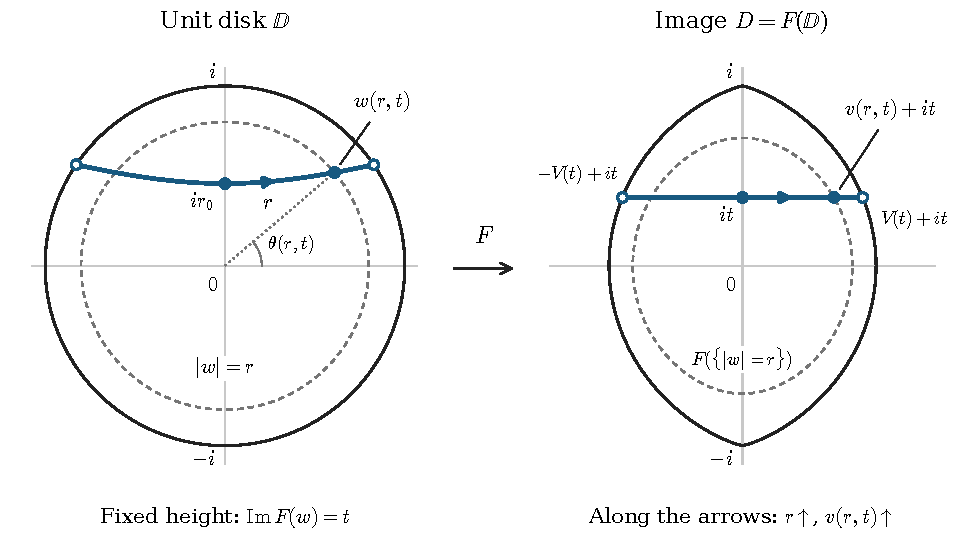
\includegraphics[width=\linewidth]{figures/lens-slices.pdf}
  \caption{A fixed horizontal slice and its preimage, illustrated for $t>0$.
  Along the right half of the highlighted preimage curve in the left panel,
  $r$ increases from
  $r_0=T^{-1}(t)$ to $1$, while $v(r,t)$ increases from $0$ to $V(t)$.
  The dashed circle and its image pass through the corresponding marked
  points. Open markers indicate boundary limits.}
  \label{fig:lens-slices}
\end{figure}


For an integer \(k\ge2\), define the signed slice integral
\begin{equation}\label{eq:slice-primitive}
 J_k(v,t)=k^2\int_0^v
       |g(h+it)|^{2k-2}|g'(h+it)|^2\,dh,
 \qquad v+it\in D.
\end{equation}
The segment of integration lies in \(D\) by Lemma~\ref{lem:planar-map}.

\begin{proposition}\label{prop:uniform-slice}
Each \(J_k\) is smooth on \(D\), is odd in \(v\), and satisfies
\begin{equation}\label{eq:slice-derivative}
 \partial_v J_k(v,t)
    =k^2|g(v+it)|^{2k-2}|g'(v+it)|^2\ge0.
\end{equation}
There is a sequence \(\epsilon_k\ge0\), depending only on \(F\), with
\(\epsilon_k\to0\) such that, simultaneously for every \(v+it\in D\),
\begin{equation}\label{eq:uniform-slice}
 \frac{|J_k(v,t)|}{k}
    \le\frac{\pi}{4}|g(v+it)|^{2k}+\epsilon_k.
\end{equation}
\end{proposition}

\begin{proof}
\noindent\textit{Step 1: express the slice integral in the disk radius.}
For any fixed \(v+it\in D\), the horizontal segment from \(it\) to
\(v+it\) is a compact subset of the open set \(D\); the same is true
for all sufficiently nearby endpoints and heights.  The formula
\[
 J_k(v,t)=k^2v\int_0^1
       |g(av+it)|^{2k-2}|g'(av+it)|^2\,da
\]
then proves smoothness by differentiation under the integral.
The integrand is smooth even at the zero of \(g\), since
\(|g|^{2k-2}=(|g|^2)^{k-1}\) and \(k\) is an integer.
Equation~\eqref{eq:slice-derivative} follows from the fundamental theorem
of calculus.  The symmetry
\(g(-\overline\zeta)=-\overline{g(\zeta)}\) makes the density in
Equation~\eqref{eq:slice-primitive} even in its real coordinate.  Thus
\(J_k(-v,t)=-J_k(v,t)\), and it suffices to estimate \(v>0\).

Fix such a point and put
\[
 R=|g(v+it)|,\qquad r_0=T^{-1}(|t|).
\]
Along its positive horizontal slice, the radius increases from \(r_0\)
to \(R\).  Since \(g'(F(w))=1/F'(w)\),
Equation~\eqref{eq:horizontal-radius-derivative} gives
\begin{equation}\label{eq:slice-radial-integral}
 \frac{J_k(v,t)}{k}
    =k\int_{r_0}^{R}
       \frac{r^{2k-1}}{A(r,\theta(r,t))}\,dr.
\end{equation}
Indeed, \(|g'|^2\,dv=(r/A)\,dr\).
At the lower endpoint this is understood as an improper integral:
perform the change of variables first on a segment beginning at a
positive real coordinate, and then let that coordinate decrease to zero.
The original integrand is smooth on the full compact segment, so its
integral is finite; the nonnegative transformed integrals converge to
the same value.  This argument also covers \(t=0\), when \(r_0=0\).

The leading constant comes from splitting \(1/A\) into \(\pi/2\) and
the nonnegative excess \(1/A-\pi/2\), since \(0<A<2/\pi\).
The constant part in Equation~\eqref{eq:slice-radial-integral} contributes
\(\frac{\pi}{4}(R^{2k}-r_0^{2k})\).  It therefore suffices to bound
the remaining weighted integral uniformly over all heights and endpoints
by a quantity tending to zero as \(k\to\infty\).

\medskip
\noindent\textit{Step 2: estimate the loss near the two tips.}
We next control the possible small denominator near the ends of the
right semicircle.  Suppose \(1/2\le r<1\) and set
\[
 s=\frac{\pi}{2}-|\theta|\in(0,\pi/2],
 \qquad
 X=\frac{2r\sin s}{1-r^2}.
\]
For every \(X>0\),
\begin{equation}\label{eq:reciprocal-arctan}
 \frac{1}{\arctan X}-\frac{2}{\pi}\le\frac{2}{X}.
\end{equation}
For \(X\le1\), this follows from \(\arctan X\ge X/2\); for \(X\ge1\),
use \(\pi/2-\arctan X=\arctan(1/X)\le1/X\) and
\(\arctan X\ge\pi/4\).  Combining
Equation~\eqref{eq:reciprocal-arctan} with
\(\sin s\ge2s/\pi\) and \((1+r)/(2r)\le3/2\), we obtain
\begin{equation}\label{eq:A-angular-bound}
 \frac1{A(r,\theta)}
    \le\frac{\pi}{2}+\frac{3\pi^3}{8}\frac{1-r}{s}.
\end{equation}
On the other hand, the vertical gap to the semicircle endpoint is
\begin{align}
 \Delta(r,\theta)
   &:=T(r)-|\Im F(re^{i\theta})|
     =\int_0^s\frac{4}{\pi^2}
          \arctan\frac{2r\sin\xi}{1-r^2}\,d\xi \notag\\
   &\le\frac{4r}{\pi^2(1-r^2)}s^2
     \le\frac{2}{\pi^2}\frac{s^2}{1-r}.
 \label{eq:vertical-gap}
\end{align}
Here we used \(\arctan y\le y\) and \(\sin\xi\le\xi\).
The last inequality supplies the lower bound
\(s\ge(\pi/\sqrt2)\sqrt{\Delta(r,\theta)(1-r)}\).
Consequently, with the absolute constant
\(C_0=3\sqrt2\pi^2/8\), Equation~\eqref{eq:A-angular-bound} implies
\begin{equation}\label{eq:A-slice-bound}
 \frac1{A(r,\theta(r,t))}
   \le\frac{\pi}{2}
        +C_0\sqrt{\frac{1-r}{T(r)-|t|}}
 \qquad (r\ge1/2,\ r>r_0).
\end{equation}

\medskip
\noindent\textit{Step 3: separate a compact part from the tip region.}
Fix a radius \(r_*\in(1/2,1)\).  The part of the original horizontal
integral for which \(|g|\le r_*\) is uniformly bounded, after division
by \(k\), by
\begin{equation}\label{eq:slice-inner-bound}
 C_*k r_*^{2k-2},
 \qquad
 C_*:=\operatorname{diam}(D)
          \max_{|w|\le r_*}|F'(w)|^{-2}<\infty.
\end{equation}
To see this, the radius is strictly increasing along the positive
slice, so the relevant portion is exactly its initial segment ending
at radius \(\min(R,r_*)\), when \(r_0\le r_*\), and is empty otherwise.
Every point of this segment lies in \(F(\{|w|\le r_*\})\), and its
horizontal length is at most \(\operatorname{diam}(D)\).
This includes the case \(R\le r_*\), when it is the whole integral.

If an outer portion remains, put
\[
 r_a=\max(r_0,r_*),\qquad
 L_*:=\inf_{r_*\le r<1}T'(r)>0.
\]
Since \(T(r_a)\ge T(r_0)=|t|\), for \(r>r_a\) we have
\begin{equation}\label{eq:gap-tail-bound}
 T(r)-|t|\ge T(r)-T(r_a)\ge L_*(r-r_a).
\end{equation}
Equations~\eqref{eq:slice-radial-integral} and
\eqref{eq:A-slice-bound} therefore bound the outer contribution by
\begin{equation}\label{eq:slice-outer-bound}
 \frac{\pi}{4}\bigl(R^{2k}-r_a^{2k}\bigr)
  +\frac{C_0}{\sqrt{L_*}}\,
       k\int_{r_a}^{1}r^{2k-1}
                 \sqrt{\frac{1-r}{r-r_a}}\,dr.
\end{equation}
The extension of the error integral from \(R\) to \(1\) uses its
nonnegativity and removes any dependence on the distance \(R-r_a\).

The last integral has an absolute bound, including when its lower
endpoint depends on \(k\).  Write
\[
 I(k,r_a)=k\int_{r_a}^{1}r^{2k-1}
                    \sqrt{\frac{1-r}{r-r_a}}\,dr,
 \qquad H=k(1-r_a).
\]
The substitution \(y=k(1-r)\) gives
\begin{align*}
 I(k,r_a)
   &=\int_0^H(1-y/k)^{2k-1}\sqrt{\frac{y}{H-y}}\,dy\\
   &\le\int_0^H e^{-y}\sqrt{\frac{y}{H-y}}\,dy,
\end{align*}
since \(\log r\le-(1-r)\) and \(2k-1\ge k\).
On \([0,H/2]\) the square-root factor is at most one.  On
\([H/2,H]\), bound the exponential by \(e^{-H/2}\) and use
\[
 \int_0^H\sqrt{\frac{y}{H-y}}\,dy=\frac{\pi H}{2}.
\]
It follows that
\begin{equation}\label{eq:uniform-endpoint-integral}
 I(k,r_a)\le 1+\frac{\pi H}{2}e^{-H/2}
           \le 1+\frac{\pi}{e}.
\end{equation}
The same integral without its exponential factor also gives
\(I(k,r_a)\le\pi H/2\).  These estimates hold for every \(H>0\),
covering both \(H\downarrow0\) and \(H\to\infty\).

Combining Equations~\eqref{eq:slice-inner-bound},
\eqref{eq:slice-outer-bound}, and
\eqref{eq:uniform-endpoint-integral}, and using symmetry when \(v<0\),
we have, for every \(v+it\in D\),
\begin{equation}\label{eq:slice-uniform-error-bound}
 \frac{|J_k(v,t)|}{k}-\frac{\pi}{4}|g(v+it)|^{2k}
   \le C_*k r_*^{2k-2}
          +\frac{C_0(1+\pi/e)}{\sqrt{L_*}}.
\end{equation}
When there is no outer portion, the first term alone bounds the excess,
so the same displayed inequality remains valid.  It is also valid at
\(v=0\).

\medskip
\noindent\textit{Step 4: make the error uniform.}
The cutoff radius will be chosen before the power $k$, so the estimates
above allow the slice height and both radial endpoints to move with $k$.
Define explicitly
\begin{equation}\label{eq:slice-error-sequence}
 \epsilon_k=
 \max\left\{0,\ \sup_{v+it\in D}
     \left(\frac{|J_k(v,t)|}{k}
                  -\frac{\pi}{4}|g(v+it)|^{2k}\right)\right\}.
\end{equation}
Equation~\eqref{eq:slice-uniform-error-bound} makes this supremum finite
for each \(k\).  For fixed \(r_*\), its first error term tends to zero
as \(k\to\infty\).  Moreover, Equation~\eqref{eq:planar-T} gives
\[
 L_*\ge\frac{8}{\pi^2}\operatorname{arctanh}r_*
       \longrightarrow\infty
 \qquad\text{as }r_*\uparrow1.
\]
Given \(\varepsilon>0\), first choose \(r_*\) so that the second term
in Equation~\eqref{eq:slice-uniform-error-bound} is less than
\(\varepsilon/2\).  For this fixed \(r_*\), choose \(N\) such that
\(C_*k r_*^{2k-2}<\varepsilon/2\) for every \(k\ge N\).
The resulting bound \(\epsilon_k<\varepsilon\) holds simultaneously
on all of \(D\).  In particular it allows the height \(t\), the initial
radius \(r_0\), and the final radius \(R\) all to vary with \(k\), with
no separation from either endpoint.  This proves
\(\epsilon_k\to0\) and Equation~\eqref{eq:uniform-slice}.
\end{proof}

\section{Realization in a polar product}
\label{sec:realization}

We now combine the ball construction with the uniform slice estimate.
Writing \(z=u+ix\), the imaginary coordinates \(x\) will give the position
in a convex body.  The signed slice integrals will correct the standard
momentum \(-u\) to account for the holomorphic part of the symplectic form.

\begin{proposition}\label{prop:finite-strips}
Let $n\ge2$ be an integer, let $b_1,\ldots,b_m\in\R^n$ span $\R^n$,
and set
\[
 K=\{x\in\R^n: |b_j\cdot x|\le 1,
                         \quad 1\le j\le m\}.
\]
For every $0<c<4$ there is a smooth symplectic embedding
\[
 B^{2n}(c)\longrightarrow
 \interior(K)\times\interior(K^\circ).
\]
\end{proposition}

\begin{proof}
\noindent\textit{Step 1: encode the strips by holomorphic functions.}
The body $K$ and its finite list of defining vectors are fixed throughout
the proof. Extend each real functional $b_j\cdot x$ complex-linearly to
$\ell_j(z)=b_j\cdot z$. Let $F:\D\to D$ and $g=F^{-1}$ be the maps of
Lemma~\ref{lem:planar-map}, and define
\begin{equation}\label{eq:strip-domain}
 \Omega=\{z\in\C^n:\ell_j(z)\in D\text{ for every }j\}.
\end{equation}
This is an open neighborhood of the origin. The spanning condition makes
the linear map $z\mapsto(\ell_1(z),\ldots,\ell_m(z))$ injective, so there
is a constant $C_b$ such that
\[
 |z|\le C_b\max_j|\ell_j(z)|.
\]
Since $D$ is bounded, $\Omega$ is bounded as well; neither set depends on
the integer $k$ chosen below. The same linear bound makes $K$ compact,
and a sufficiently small Euclidean ball lies in all its defining strips.
In particular, $0\in\interior(K)$.

For each integer $k\ge2$, put
\[
 f_j(z)=g(\ell_j(z))^k,\qquad
 \tau(z)=\sum_{j=1}^m|f_j(z)|^2,\qquad
 V=\{z\in\Omega:\tau(z)<1\},\qquad
 \omega=\ddc\bigl(|z|^2+\tau\bigr).
\]
The tuple $f=(f_1,\ldots,f_m)$ is holomorphic on $\Omega$. Since $g$ has
its only zero at the origin, the common zero set of $f$ is
\[
 \{z\in\Omega:\ell_j(z)=0\text{ for every }j\}=\{0\}.
\]
Holomorphicity at the origin gives $|f(z)|=O(|z|^k)$. To verify the
compactness hypothesis of Theorem~\ref{thm:holomorphic-ball}, fix
$0<s<1$. On $\{\tau\le s\}$, for every $j$ we have
\[
 \ell_j(z)\in
 F\bigl(\{w\in\C:|w|\le s^{1/(2k)}\}\bigr),
\]
a compact subset of $D$. The linear bound above makes this sublevel
bounded. Moreover, the limit of any convergent sequence in it still has
all its images under the functionals $\ell_j$ in that compact subset
of $D$, hence belongs to
$\Omega$ and satisfies $\tau\le s$ by continuity. Thus the sublevel is
compact in $\Omega$. Theorem~\ref{thm:holomorphic-ball} now supplies
symplectic embeddings into $(V,\omega)$ of every standard ball of
capacity less than $\pi k$.

\medskip
\noindent\textit{Step 2: realize the form by a globally injective map.}
Write $z=u+ix$ and use the signed integrals $J_k$ of
Proposition~\ref{prop:uniform-slice} to define
\begin{equation}\label{eq:strip-phase-map}
 \Phi_k:V\longrightarrow\R^n_q\times\R^n_p,
 \qquad
 q=x,\qquad
 p=-u-\sum_{j=1}^m
       J_k(b_j\cdot u,b_j\cdot x)b_j.
\end{equation}
The signed integrals $J_k$ are smooth on $D$ by
Proposition~\ref{prop:uniform-slice}, so $\Phi_k$ is smooth.

Set $v_j=b_j\cdot u$ and $t_j=b_j\cdot x$. Pulling back the target
form gives
\begin{align}
 \Phi_k^*\omega_0
 &=\sum_{\ell=1}^n dx_\ell\wedge(-du_\ell)
       -\sum_{j=1}^m dt_j\wedge dJ_k(v_j,t_j)\notag\\
 &=\sum_{\ell=1}^n du_\ell\wedge dx_\ell
       +\sum_{j=1}^m
          \partial_vJ_k(v_j,t_j)\,dv_j\wedge dt_j\notag\\
 &=\ddc\bigl(|z|^2+\tau\bigr)=\omega.
 \label{eq:strip-pullback}
\end{align}
Indeed, the terms containing $\partial_tJ_k$ vanish because
$dt_j\wedge dt_j=0$, while
\[
 \partial_vJ_k(v,t)=k^2|g(v+it)|^{2k-2}|g'(v+it)|^2.
\]
This is precisely the coefficient of $\ddc|g(v+it)^k|^2$ in front of
$dv\wedge dt$, with the convention for $\dc$ fixed above.

The map $\Phi_k$ is globally injective. To see this, equality of its
$q$ coordinates first fixes $x$. For two possible real coordinates
$u_1,u_2$ at that $x$, write
\[
 \Delta u=u_2-u_1,\qquad
 v_{ji}=b_j\cdot u_i,\qquad t_j=b_j\cdot x,
\]
and denote the corresponding momenta by $p_1,p_2$. Both $v_{j1}$ and
$v_{j2}$ belong to the same horizontal interval of $D$ at height $t_j$.
Since $\partial_vJ_k\ge0$ on this entire interval,
\begin{align*}
 (p_2-p_1)\cdot\Delta u
 &=-|\Delta u|^2
   -\sum_{j=1}^m
     \bigl(J_k(v_{j2},t_j)-J_k(v_{j1},t_j)\bigr)
     (v_{j2}-v_{j1})\\
 &\le -|\Delta u|^2.
\end{align*}
Thus equal momenta force $u_1=u_2$. This comparison applies to any two
points of the fiber, even if that fiber of $V$ is disconnected.
Equation~\eqref{eq:strip-pullback} and nondegeneracy of $\omega$ show that
$\Phi_k$ is a local diffeomorphism. It is therefore open, and its
injectivity gives a smooth inverse onto its image. Consequently
$\Phi_k$ is a symplectic embedding.

\medskip
\noindent\textit{Step 3: control the momentum by the polar body.}
We next bound its image. All imaginary parts of points of $D$ lie in
$(-1,1)$, so $|b_j\cdot x|<1$ for every $j$. The finite system of
strict inequalities implies $q=x\in\interior(K)$. Introduce the support
function
\[
 h_K(p)=\max_{y\in K}\ip{p}{y}.
\]
It satisfies $h_K(\pm b_j)\le1$, and
$\interior(K^\circ)=\{p:h_K(p)<1\}$. Because $\Omega$ is bounded,
there is a finite constant $C_K$, independent of $k$, such that
$h_K(-u)\le C_K$ on $\Omega$. Subadditivity and positive homogeneity of
$h_K$, followed by Proposition~\ref{prop:uniform-slice}, give
\begin{align}
 \frac{h_K(p)}{k}
 &\le \frac{C_K}{k}
       +\sum_{j=1}^m\frac{|J_k(v_j,t_j)|}{k}\notag\\
 &\le \frac{C_K}{k}
       +\frac{\pi}{4}\sum_{j=1}^m|g(\ell_j(z))|^{2k}
       +m\epsilon_k
  =\frac{C_K}{k}+\frac{\pi}{4}\tau(z)+m\epsilon_k.
 \label{eq:strip-support}
\end{align}
Here $\epsilon_k\ge0$ tends to zero, uniformly in the planar argument.
The number $m$ and the constant $C_K$ are fixed before $k$ varies.
It follows that, for any $\eta>0$ and all sufficiently large $k$,
\[
 \frac{C_K}{k}+m\epsilon_k<\frac{\eta\pi}{4}.
\]
Since $\tau<1$ on $V$, Equation~\eqref{eq:strip-support} then gives the
strict inclusion
\begin{equation}\label{eq:strip-scaled-image}
 \Phi_k(V)\subset
 \interior(K)\times S\interior(K^\circ),
 \qquad S=(1+\eta)\frac{\pi k}{4}.
\end{equation}

\medskip
\noindent\textit{Step 4: rescale the ball and the momentum together.}
Finally, fix $0<c<4$. Choose $\eta>0$ with $(1+\eta)c<4$, and then fix
an integer $k$ large enough for Equation~\eqref{eq:strip-scaled-image}.
The resulting constant $S$ satisfies $Sc<\pi k$, so there is a
symplectic embedding
\[
 E:B^{2n}(Sc)\longrightarrow(V,\omega).
\]
Let $D_{\sqrt S}(z)=\sqrt S\,z$ and
$L_S(q,p)=(q,p/S)$. The composition
\begin{equation}\label{eq:strip-rescaling}
 L_S\circ\Phi_k\circ E\circ D_{\sqrt S}:
 B^{2n}(c)\longrightarrow
 \interior(K)\times\interior(K^\circ)
\end{equation}
is a smooth embedding. Since $D_{\sqrt S}$ maps $B^{2n}(c)$ onto
$B^{2n}(Sc)$ and
\[
 D_{\sqrt S}^*\omega_0=S\omega_0,
 \qquad L_S^*\omega_0=S^{-1}\omega_0,
\]
its pullback of $\omega_0$ is exactly $\omega_0$. This proves the
proposition.
\end{proof}

\section{Arbitrary convex bodies and consequences}
\label{sec:approximation}

The passage from finite strip bodies to arbitrary convex bodies uses an
approximation in the polar. This keeps the momentum factor inside the
desired polar and enlarges the position factor by an arbitrarily small
amount.

\begin{lemma}[Finite polar approximation]
\label{lem:polar-approximation}
Let $K\subset\R^n$ be an origin-symmetric convex body. For every
$\alpha>0$, there are finitely many vectors
$b_1,\ldots,b_m\in\R^n$ spanning $\R^n$ such that
\[
 K'=\{x\in\R^n:|\ip{b_j}{x}|\le1,\quad 1\le j\le m\}
\]
satisfies
\begin{equation}\label{eq:polar-approximation}
 K\subset K'\subset(1+\alpha)K,
 \qquad (K')^\circ\subset K^\circ.
\end{equation}
\end{lemma}

\begin{proof}
First, $0\in\interior K$. Indeed, if the Euclidean ball $B(y,r)$
is contained in $K$, then so is $B(-y,r)$, and their midpoints contain
$B(0,r)$. Since $K$ is also bounded, there are $r,R>0$ with
$B(0,r)\subset K\subset B(0,R)$. The definition of the polar gives
\[
 B(0,R^{-1})\subset K^\circ\subset\overline{B(0,r^{-1})}.
\]
Thus $K^\circ$ is a compact, origin-symmetric convex body with nonempty
interior.

We will use the bipolar identity $K^{\circ\circ}=K$. To recall its
justification here, if $x\notin K$, separation gives a nonzero vector
$v$ such that
\[
 \ip{v}{x}>h_K(v),
 \qquad h_K(v)=\max_{y\in K}\ip{v}{y}>0.
\]
The normalized vector $v/h_K(v)$ belongs to $K^\circ$ and pairs with
$x$ to a value greater than $1$, so $x\notin K^{\circ\circ}$.
The reverse inclusion follows directly from the definition. The same
argument applies to every convex body containing the origin in its
interior.

Put $\lambda=1+\alpha$ and
\[
 \rho=\min_{|v|=1}h_{K^\circ}(v)>0.
\]
Choose $d>0$ with $d\le\alpha\rho/(1+\alpha)$, and choose a finite
$d$-net $\{b_1,\ldots,b_m\}$ in the compact set $K^\circ$, with all
net points in $K^\circ$. Let
\[
 P=\operatorname{conv}\{\pm b_1,\ldots,\pm b_m\}.
\]
Symmetry of $K^\circ$ gives $P\subset K^\circ$. For every unit vector
$v$, a maximizer of $\ip{v}{p}$ over $p\in K^\circ$ lies within
distance $d$ of a net point. Consequently
\[
 h_P(v)\ge h_{K^\circ}(v)-d
       \ge\lambda^{-1}h_{K^\circ}(v).
\]
The characterization of inclusion by support functions, which follows
from convex separation, now gives
\[
 \lambda^{-1}K^\circ\subset P\subset K^\circ.
\]
In particular, $P$ has interior, so its generating vectors span
$\R^n$. Taking polars and using the bipolar identity yields
\[
 K\subset P^\circ\subset\lambda K,
 \qquad (P^\circ)^\circ=P\subset K^\circ.
\]
Finally, the definition of $P$ shows that $P^\circ$ is exactly the
finite strip body $K'$ in the statement.
\end{proof}

\begin{proof}[Proof of Theorem~\ref{thm:main}]
Fix $0<c<4$. Choose $\alpha>0$ such that $\lambda c<4$, where
$\lambda=1+\alpha$, and choose one body $K'$ from
Lemma~\ref{lem:polar-approximation}. Proposition~\ref{prop:finite-strips}
gives a smooth symplectic embedding
\[
 e:B^{2n}(\lambda c)\longrightarrow
 \interior K'\times\interior\bigl((K')^\circ\bigr).
\]
If one body is contained in another, every interior ball in the first
is contained in the second. Thus Equation~\eqref{eq:polar-approximation}
implies
\[
 \interior K'\subset\lambda\interior K,
 \qquad \interior\bigl((K')^\circ\bigr)\subset\interior K^\circ,
\]
even when their boundaries meet. Regard $e$ as an embedding into
$\lambda\interior K\times\interior K^\circ$. Define
\[
 D_{\sqrt\lambda}(z)=\sqrt\lambda\,z,
 \qquad Q_\lambda(q,p)=(q/\lambda,p).
\]
The composition
\begin{equation}\label{eq:general-rescaling}
 Q_\lambda\circ e\circ D_{\sqrt\lambda}:
 B^{2n}(c)\longrightarrow U_K
\end{equation}
is a smooth embedding. Since
\[
 D_{\sqrt\lambda}^*\omega_0=\lambda\omega_0,
 \qquad Q_\lambda^*\omega_0=\lambda^{-1}\omega_0,
\]
its pullback of $\omega_0$ equals $\omega_0$. This proves
$c_G(U_K)\ge4$.

For the upper bound, we use the supporting-slab construction of
Artstein-Avidan, Karasev, and Ostrover
\cite[Remark~4.2]{AAKO2014}. Choose $q_0\in K$ and $p_0\in K^\circ$
with $\ip{q_0}{p_0}=1$. Such a pair is obtained by maximizing any
nonzero linear functional on $K$ and normalizing its maximum to $1$.
Complete $q_0$ to a basis of $\R^n$ by vectors in $\ker p_0$, and let
$A$ be the matrix of this basis. The linear change
\[
 Q=A^{-1}q,\qquad P=A^Tp
\]
is symplectic and has first coordinates
$Q_1=\ip{p_0}{q}$ and $P_1=\ip{q_0}{p}$.
Both functionals are nonzero, so symmetry, polarity, and the interior
condition give $|Q_1|<1$ and $|P_1|<1$ on $U_K$.
Thus this change embeds $U_K$ into
$(-1,1)^2\times\R^{2n-2}$, with the square in its first conjugate
coordinate pair.

For completeness, this open square is area-preservingly diffeomorphic
to the disk of area $4$. Put $R=2/\sqrt\pi$,
$h(X)=\sqrt{R^2-X^2}$ for $-R<X<R$, and
\[
 H(X)=-1+\int_{-R}^{X}h(s)\,ds.
\]
Since $\int_{-R}^{R}h(s)\,ds=2$ and $H'=h>0$,
$H$ is a smooth diffeomorphism from $(-R,R)$ onto $(-1,1)$.
The map
\[
 (u,v)\longmapsto
 \bigl(X=H^{-1}(u),\ Y=v\,h(H^{-1}(u))\bigr)
\]
has image $B^2(4)$ and Jacobian $X'(u)h(X)=1$.
Applying it to the first conjugate pair gives a symplectic embedding
$U_K\hookrightarrow B^2(4)\times\R^{2n-2}$.
Gromov's nonsqueezing theorem \cite{Gromov1985} therefore bounds the
capacity of every ball in $U_K$ by $4$. Combined with the lower bound,
this proves $c_G(U_K)=4$.
\end{proof}

\begin{remark}[Order of choices]
\label{rem:parameter-order}
For each prescribed $0<c<4$, first choose $\alpha>0$ so that
$\lambda c<4$, where $\lambda=1+\alpha$. Then fix the finite body
$K'$ and its $m$ defining constraints. Choose $\eta>0$ so that
$(1+\eta)\lambda c<4$, then choose $k$ large enough that
\[
 \frac{C_{K'}}k+m\epsilon_k<\frac{\eta\pi}{4}.
\]
This is possible because the constraint list is fixed before $k$
varies. Proposition~\ref{prop:finite-strips}, applied at capacity
$\lambda c$, and the final rescaling then give the required ball.
Each prescribed capacity is obtained by one finite construction; no
limit of embeddings is required.
\end{remark}

\begin{corollary}[Symmetric Mahler inequality]
\label{cor:mahler}
For every integer $n\ge1$ and every origin-symmetric convex body
$K\subset\R^n$,
\[
 \vol_n(K)\,\vol_n(K^\circ)\ge\frac{4^n}{n!}.
\]
\end{corollary}

\begin{proof}
For $n=1$, write $K=[-a,a]$ with $a>0$. Then
$K^\circ=[-a^{-1},a^{-1}]$, and the product of their lengths is $4$.
Assume henceforth that $n\ge2$.

We first justify that taking interiors does not change the volumes in
the statement. If a convex body $C\subset\R^n$ contains $B(0,r)$,
then convexity gives, for $0<t<1$,
\[
 tC+B(0,(1-t)r)\subset C.
\]
Hence $tC\subset\interior C$, and
\[
 t^n\vol_n(C)\le\vol_n(\interior C)\le\vol_n(C).
\]
Letting $t\uparrow1$ proves
$\vol_n(\interior C)=\vol_n(C)$. Apply this to $K$ and $K^\circ$,
both of which contain a neighborhood of the origin. The product formula
for Lebesgue measure then gives
\begin{equation}\label{eq:polar-product-volume}
 \vol_{2n}(U_K)=\vol_n(K)\,\vol_n(K^\circ).
\end{equation}

For every $0<c<4$, Theorem~\ref{thm:main} supplies a smooth symplectic
embedding $f:B^{2n}(c)\to U_K$. Taking the $n$th exterior power of
$f^*\omega_0=\omega_0$ shows that $\det Df=1$, so the change of
variables formula gives
\[
 \frac{c^n}{n!}
 =\vol_{2n}\bigl(B^{2n}(c)\bigr)
 =\vol_{2n}\bigl(f(B^{2n}(c))\bigr)
 \le\vol_{2n}(U_K).
\]
Here the first equality follows from the Euclidean ball volume
$\pi^nR^{2n}/n!$ at radius $R=\sqrt{c/\pi}$. Combining this with
Equation~\eqref{eq:polar-product-volume} and letting $c\uparrow4$ proves
the claimed inequality.
\end{proof}

\begin{remark}[Sharpness]
The cube $[-1,1]^n$ has volume $2^n$. Its polar is
$\{p:\sum_{j=1}^n|p_j|\le1\}$, whose intersection with each coordinate
orthant is a simplex of volume $1/n!$. These $2^n$ simplices meet only
along faces, so the polar has volume $2^n/n!$. Their volume product is
therefore $4^n/n!$, showing that the constant in
Corollary~\ref{cor:mahler} is sharp.
\end{remark}

\begin{corollary}[A sufficient packing criterion]
\label{cor:polar-packings}
Let $n\ge3$ and $k\ge1$ be integers, and let $K\subset\R^n$ be an
origin-symmetric convex body. Suppose that $R_1,\ldots,R_k>0$ satisfy
\[
 \sum_{i=1}^k R_i^n<4^n,
 \qquad R_i+R_j<4\quad(1\le i<j\le k).
\]
Then there are symplectic embeddings of open neighborhoods of the closed
balls $\overline{B^{2n}(R_1)},\ldots,\overline{B^{2n}(R_k)}$ into $U_K$
with pairwise disjoint images. The pairwise condition is vacuous for $k=1$.
\end{corollary}

\begin{proof}
Strictness and finiteness permit a choice of $0<c<4$ such that
$\sum_i R_i^n<c^n$ and $R_i+R_j<c$ for every $i<j$.
The ball-packing theorem \cite[Theorem~1.1]{OpenAIBallPackings2026}
embeds these closed balls into $B^{2n}(c)$, with embeddings defined on
neighborhoods. Their compact images are pairwise disjoint and lie in the
open target, so the neighborhoods can be shrunk to have pairwise disjoint
images contained in $B^{2n}(c)$. Composing with the embedding in
Theorem~\ref{thm:main} proves the assertion.
\end{proof}

\begingroup
\raggedright
\let\originalthebibliography\thebibliography
\renewcommand{\thebibliography}[1]{%
  \originalthebibliography{#1}%
  \setlength{\itemsep}{2pt}%
  \addcontentsline{toc}{section}{References}%
}
\bibliographystyle{plain}
\bibliography{references}
\endgroup
\end{document}
